\documentclass{article}

\usepackage[english]{babel}
\usepackage[utf8]{inputenc}
\usepackage{amsmath,amssymb}
\usepackage{parskip}
\usepackage{graphicx}

% Margins
\usepackage[top=2.5cm, left=3cm, right=3cm, bottom=4.0cm]{geometry}
% Colour table cells
\usepackage[table]{xcolor}
\usepackage{graphicx}
% Get larger line spacing in table
\newcommand{\tablespace}{\\[1.25mm]}
\newcommand\Tstrut{\rule{0pt}{2.6ex}}         % = `top' strut
\newcommand\tstrut{\rule{0pt}{2.0ex}}         % = `top' strut
\newcommand\Bstrut{\rule[-0.9ex]{0pt}{0pt}}   % = `bottom' strut

%%%%%%%%%%%%%%%%%
%     Title     %
%%%%%%%%%%%%%%%%%
\title{Implicit Differentiation}
\author{Franco Vidal \\ Math 124}
\date{\today}

\begin{document}
\maketitle
\section{Circle Example}
For a circle with equation $x^2 + y^2=5^2$ With a Point P = (3,4), find the tangent line using implicit differentiation 
\begin{figure}[h]
\caption{$x^2 + y^2 = 5^2$ with tangent line through P}
\centering
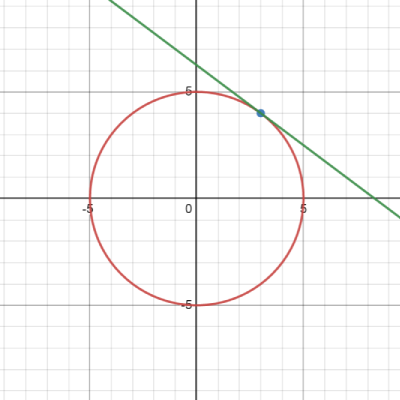
\includegraphics[width=0.5\textwidth]{Circle1.png}
\end{figure}
\begin{equation}
x^2 + y^2 = 5^2
\end{equation}
\begin{equation}
(x^2 + y^2)\frac{dy}{dx} = (5) \frac{dy}{dx}
\end{equation}
\begin{equation}
(x^2)\frac{dy}{dx} + (y^2)\frac{dy}{dx} = 0
\end{equation}
Because we're differentiating in terms of $x$, we treat $y$ differently
\begin{equation}
2x + (y^2)\frac{dy}{dx}
\end{equation}
\begin{equation}
2x + 2yy' = 0
\end{equation}
We then solve for y'
\begin{equation}
2yy' = 0 - 2x
\\\frac{2yy'}{2y}=\frac{0-2x}{2y}
\\y' = \frac{-x}{y}
\end{equation}
We then plug in P (3,4)
\begin{equation}
y'|_{(3,4)} = \frac{-3}{4} 
\end{equation}
This gives us the slope of the tangent line at P, in order to find the equation of the line, we plug it into the slope equation:
\begin{equation}
y = mx(x-x_1)+y_1
\end{equation}
\begin{equation}
y = \frac{-3}{4}(x - 3)+4
\end{equation}
\section{Ellipse Example} 
For a curve of equation $2x^2 + xy + y^2 = 4$, find the derivative
\begin{figure}[h]
\caption{$x^2 + y^2 = 5^2$ with tangent line through P}
\centering
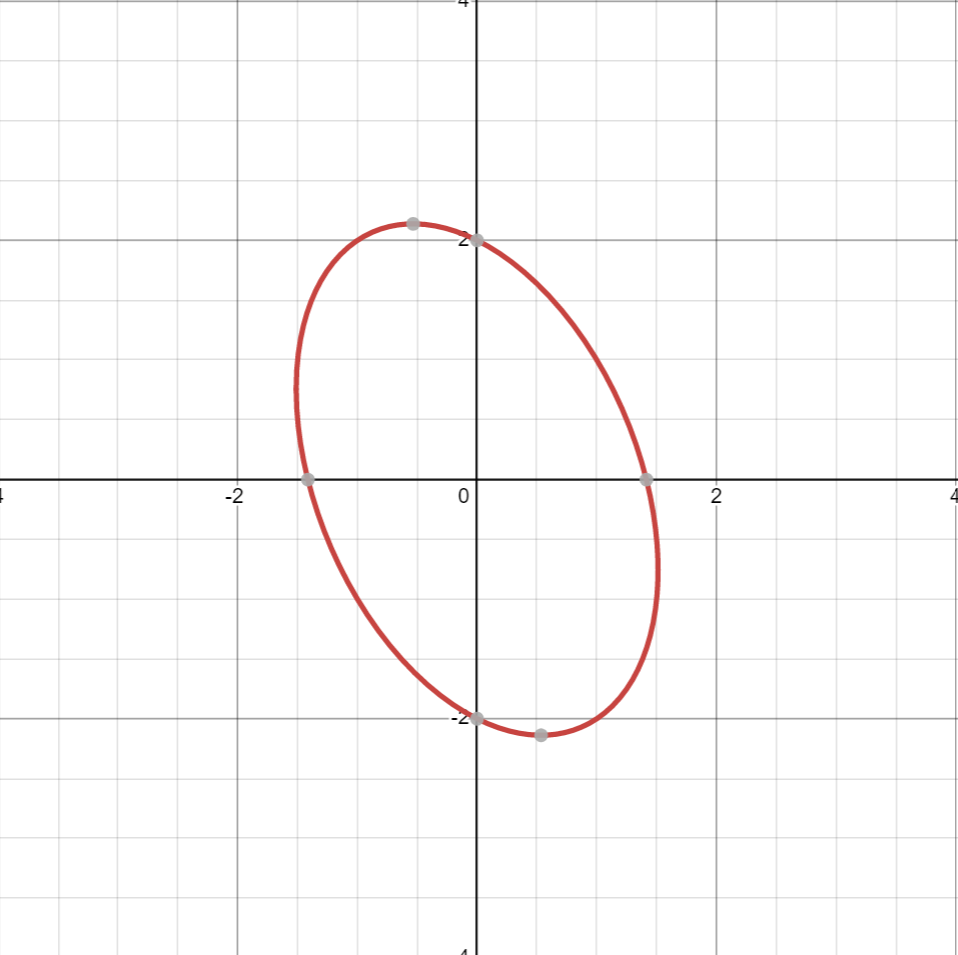
\includegraphics[width=0.5\textwidth]{Ellipse1.png}
\end{figure}
\begin{equation}
2x^2 + xy + y^2 = 4
\end{equation}
\begin{equation}
\frac{dy}{dx}(2x^2 + xy + y^2) = \frac{dy}{dx}(4)
\end{equation}
\begin{equation}
\frac{dy}{dx}(2x^2)\frac{d}{dx}(xy)+\frac{d}{dx}(y^2) = 0
\end{equation}
\begin{equation}
4x + x \frac{dy}{dx} + \frac{dy}{dx}(x)y + 2y\frac{dy}{dx} = 0
\end{equation}
\begin{equation}
4x + x \frac{dy}{dx} + y + 2y \frac{dy}{dx} = 0
\end{equation}
Move all of the numbers without a $\frac{dy}{dx}$ to the other side of the equation, then solve.
\begin{equation}
x \frac{dy}{dx} + 2y \frac{dy}{dx} = -4x-y
\end{equation}
\begin{equation}
\frac{dy}{dx}(x + 2y) = -4x-y
\end{equation}
Divide both sides by $(x+2y)$
\begin{equation}
\frac{dy}{dx} = \frac{-4x-y}{x+2y}
\end{equation}
\end{document}